\documentclass[11pt]{article}
\usepackage[textwidth=18.0cm, textheight=23.0cm, top=2.0cm]{geometry}
\usepackage{pst-all}
\usepackage{amssymb}
\usepackage{tikz}
\usepackage{underscore}\begin{document}
\pagestyle{empty}


ClassName: \underline{\textbf{Class_10.2bp-37}}
\par
BinSize: \underline{\textbf{100 × 100}}
\par
ReduceSize: \underline{\textbf{100 × 100}}
\par
TypeNum: \underline{\textbf{80}}
\par
Num: \underline{\textbf{80}}
\par
OutS: \underline{\textbf{100000}}
\par
InS: \underline{\textbf{93747}}
\par
Rate: \underline{\textbf{0.937}}
\par
UB: \underline{\textbf{10}}
\par
LB0: \underline{\textbf{10}}
\par
LB: \underline{\textbf{10}}
\par
LBWithCut: \underline{\textbf{10}}
\par
NodeCut: \underline{\textbf{0}}
\par
ExtendedNodeCnt: \underline{\textbf{1}}
\par
GenNodeCnt: \underline{\textbf{1}}
\par
PrimalNode: \underline{\textbf{0}}
\par
ColumnCount: \underline{\textbf{10}}
\par
TotalCutCount: \underline{\textbf{0}}
\par
RootCutCount: \underline{\textbf{0}}
\par
LPSolverCnt: \underline{\textbf{1}}
\par
PricingSolverCnt: \underline{\textbf{0}}
\par
BranchAndBoundNum: \underline{\textbf{1}}
\par
isOpt: \underline{\textbf{true}}
\par
TimeOnInitSolution: \underline{\textbf{600.000 s}}
\par
TimeOnPrimal: \underline{\textbf{0.000 s}}
\par
TimeOnPricing: \underline{\textbf{0.000 s}}
\par
TimeOnRmp: \underline{\textbf{0.078 s}}
\par
TotalTime: \underline{\textbf{600.328 s}}
\par
\newpage


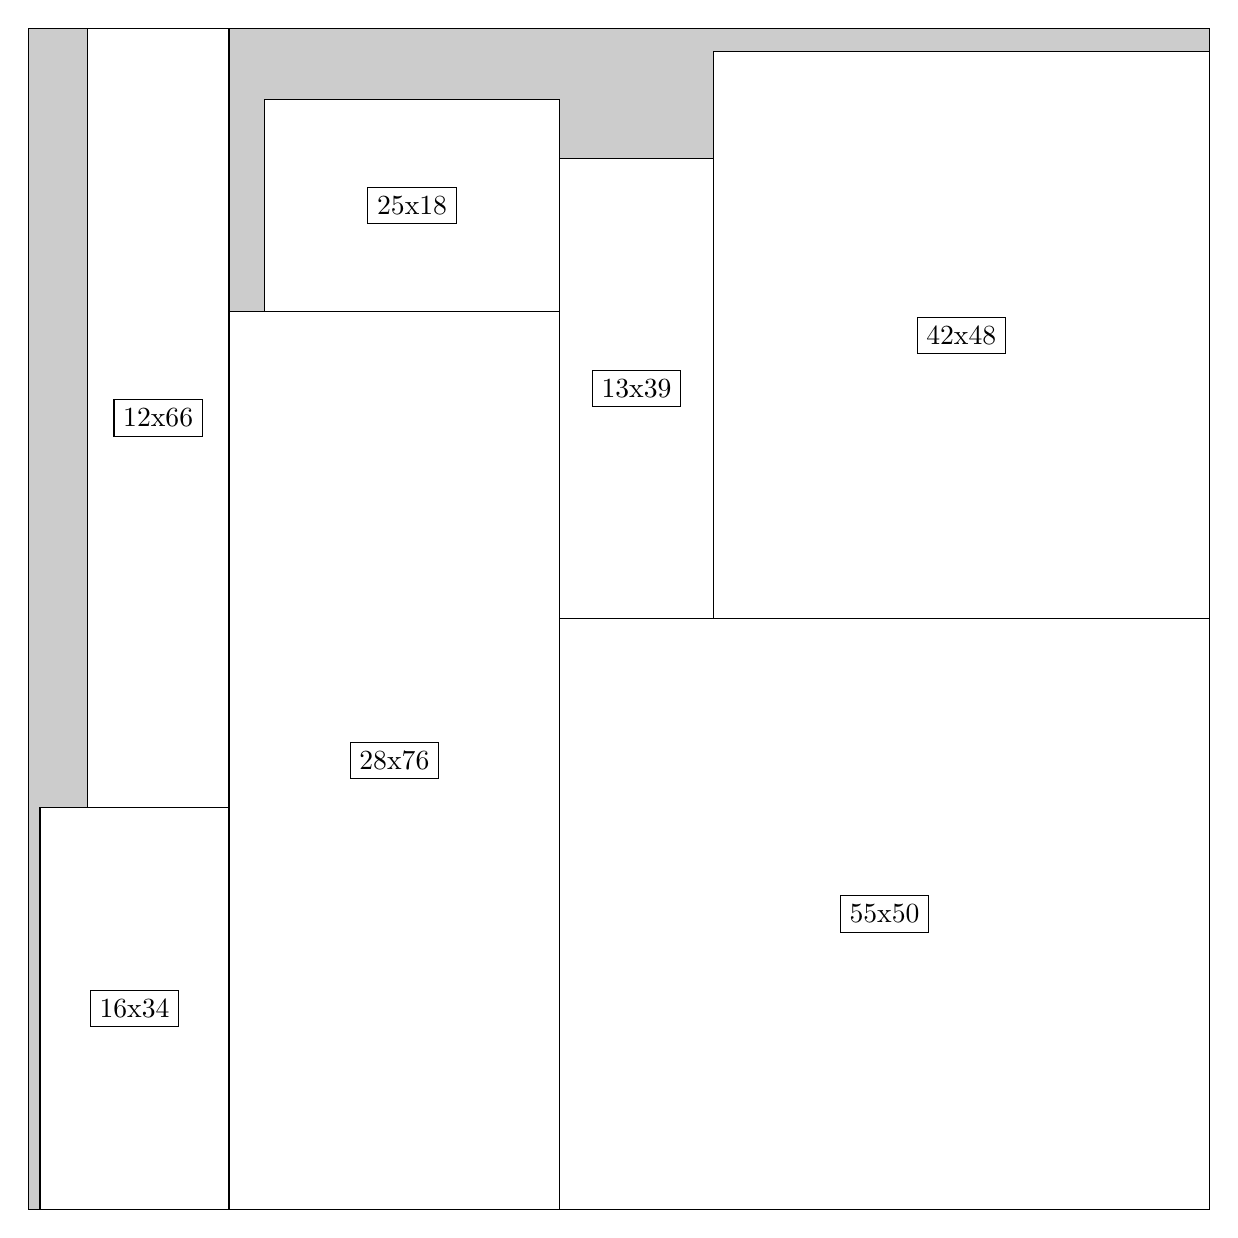
\begin{tikzpicture}[shorten >=1pt,scale=1.0,every node/.style={scale=1.0},->]
\tikzstyle{vertex}=[circle,fill=black!25,minimum size=14pt,inner sep=0pt]
\filldraw[fill=gray!40!white, draw=black] (0,0) rectangle (15.0,15.0);
\foreach \name/\x/\y/\w/\h in {55x50/6.75/0.0/8.25/7.5,42x48/8.7/7.5/6.3/7.199999999999999,13x39/6.75/7.5/1.95/5.85,28x76/2.55/0.0/4.2/11.4,25x18/3.0/11.4/3.75/2.6999999999999997,16x34/0.15/0.0/2.4/5.1,12x66/0.75/5.1/1.7999999999999998/9.9}
\filldraw[fill=white!40!white, draw=black] (\x,\y) rectangle node[draw] (\name) {\name} ++(\w,\h);
\end{tikzpicture}


w =55 , h =50 , x =45 , y =0 , v =2750
\par
w =42 , h =48 , x =58 , y =50 , v =2016
\par
w =13 , h =39 , x =45 , y =50 , v =507
\par
w =28 , h =76 , x =17 , y =0 , v =2128
\par
w =25 , h =18 , x =20 , y =76 , v =450
\par
w =16 , h =34 , x =1 , y =0 , v =544
\par
w =12 , h =66 , x =5 , y =34 , v =792
\par
\newpage


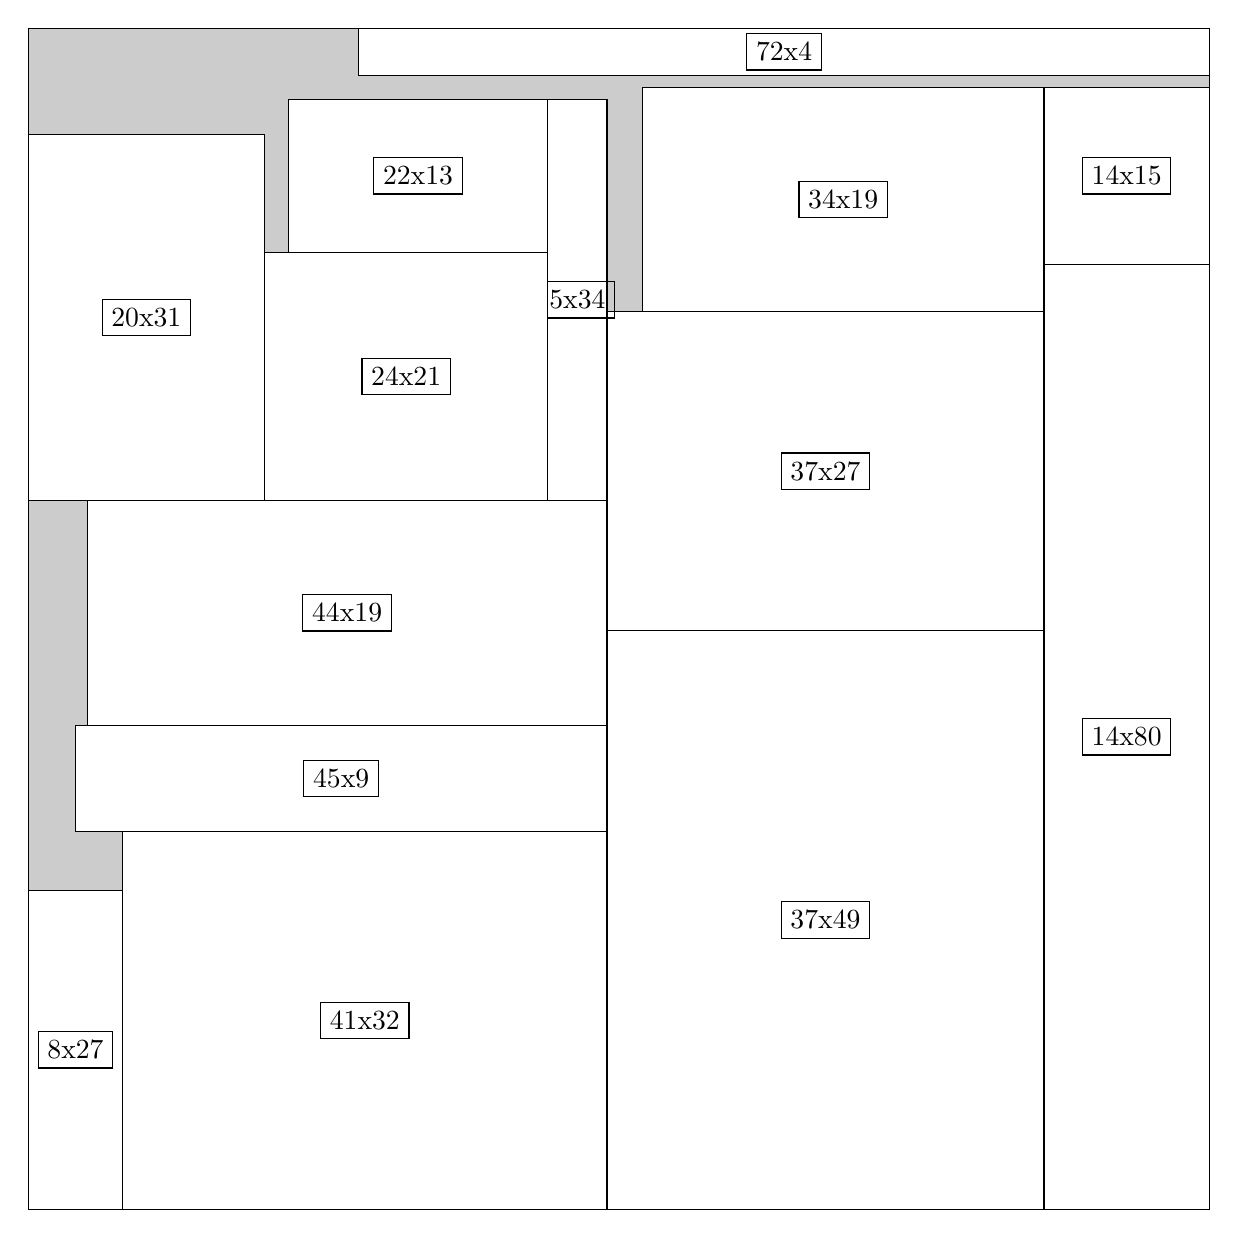
\begin{tikzpicture}[shorten >=1pt,scale=1.0,every node/.style={scale=1.0},->]
\tikzstyle{vertex}=[circle,fill=black!25,minimum size=14pt,inner sep=0pt]
\filldraw[fill=gray!40!white, draw=black] (0,0) rectangle (15.0,15.0);
\foreach \name/\x/\y/\w/\h in {14x80/12.9/0.0/2.1/12.0,14x15/12.9/12.0/2.1/2.25,37x49/7.35/0.0/5.55/7.35,37x27/7.35/7.35/5.55/4.05,34x19/7.8/11.4/5.1/2.85,41x32/1.2/0.0/6.1499999999999995/4.8,8x27/0.0/0.0/1.2/4.05,45x9/0.6/4.8/6.75/1.3499999999999999,44x19/0.75/6.1499999999999995/6.6/2.85,5x34/6.6/9.0/0.75/5.1,24x21/3.0/9.0/3.5999999999999996/3.15,22x13/3.3/12.15/3.3/1.95,20x31/0.0/9.0/3.0/4.6499999999999995,72x4/4.2/14.399999999999999/10.799999999999999/0.6}
\filldraw[fill=white!40!white, draw=black] (\x,\y) rectangle node[draw] (\name) {\name} ++(\w,\h);
\end{tikzpicture}


w =14 , h =80 , x =86 , y =0 , v =1120
\par
w =14 , h =15 , x =86 , y =80 , v =210
\par
w =37 , h =49 , x =49 , y =0 , v =1813
\par
w =37 , h =27 , x =49 , y =49 , v =999
\par
w =34 , h =19 , x =52 , y =76 , v =646
\par
w =41 , h =32 , x =8 , y =0 , v =1312
\par
w =8 , h =27 , x =0 , y =0 , v =216
\par
w =45 , h =9 , x =4 , y =32 , v =405
\par
w =44 , h =19 , x =5 , y =41 , v =836
\par
w =5 , h =34 , x =44 , y =60 , v =170
\par
w =24 , h =21 , x =20 , y =60 , v =504
\par
w =22 , h =13 , x =22 , y =81 , v =286
\par
w =20 , h =31 , x =0 , y =60 , v =620
\par
w =72 , h =4 , x =28 , y =96 , v =288
\par
\newpage


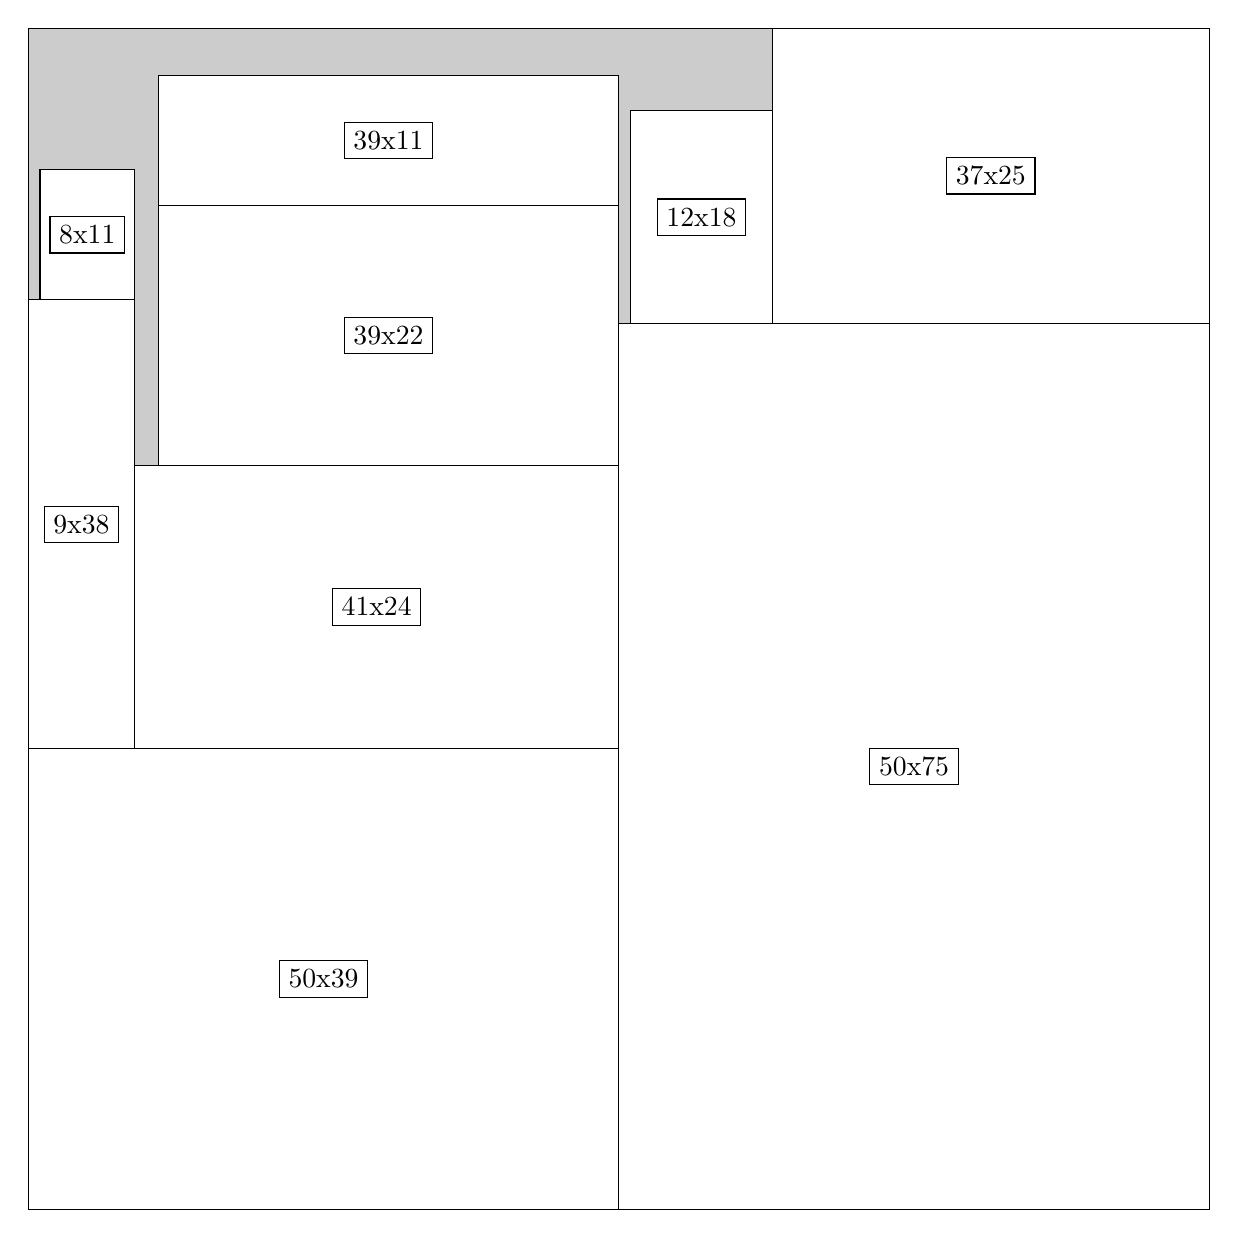
\begin{tikzpicture}[shorten >=1pt,scale=1.0,every node/.style={scale=1.0},->]
\tikzstyle{vertex}=[circle,fill=black!25,minimum size=14pt,inner sep=0pt]
\filldraw[fill=gray!40!white, draw=black] (0,0) rectangle (15.0,15.0);
\foreach \name/\x/\y/\w/\h in {50x75/7.5/0.0/7.5/11.25,37x25/9.45/11.25/5.55/3.75,12x18/7.6499999999999995/11.25/1.7999999999999998/2.6999999999999997,50x39/0.0/0.0/7.5/5.85,41x24/1.3499999999999999/5.85/6.1499999999999995/3.5999999999999996,39x22/1.65/9.45/5.85/3.3,39x11/1.65/12.75/5.85/1.65,9x38/0.0/5.85/1.3499999999999999/5.7,8x11/0.15/11.549999999999999/1.2/1.65}
\filldraw[fill=white!40!white, draw=black] (\x,\y) rectangle node[draw] (\name) {\name} ++(\w,\h);
\end{tikzpicture}


w =50 , h =75 , x =50 , y =0 , v =3750
\par
w =37 , h =25 , x =63 , y =75 , v =925
\par
w =12 , h =18 , x =51 , y =75 , v =216
\par
w =50 , h =39 , x =0 , y =0 , v =1950
\par
w =41 , h =24 , x =9 , y =39 , v =984
\par
w =39 , h =22 , x =11 , y =63 , v =858
\par
w =39 , h =11 , x =11 , y =85 , v =429
\par
w =9 , h =38 , x =0 , y =39 , v =342
\par
w =8 , h =11 , x =1 , y =77 , v =88
\par
\newpage


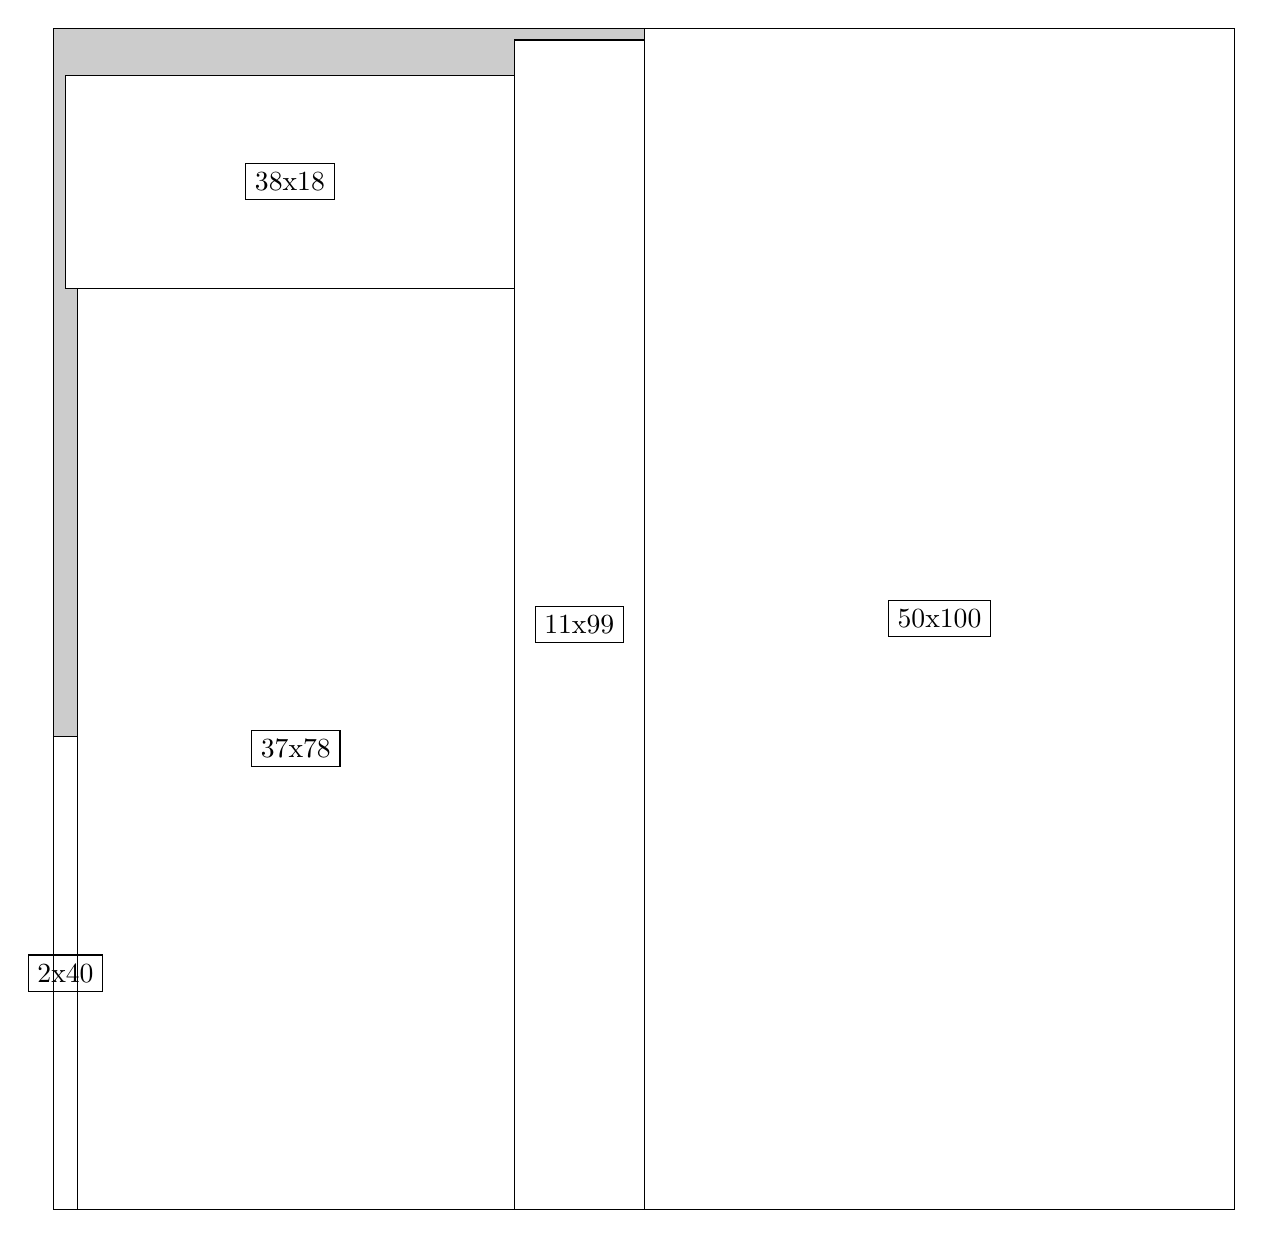
\begin{tikzpicture}[shorten >=1pt,scale=1.0,every node/.style={scale=1.0},->]
\tikzstyle{vertex}=[circle,fill=black!25,minimum size=14pt,inner sep=0pt]
\filldraw[fill=gray!40!white, draw=black] (0,0) rectangle (15.0,15.0);
\foreach \name/\x/\y/\w/\h in {50x100/7.5/0.0/7.5/15.0,11x99/5.85/0.0/1.65/14.85,37x78/0.3/0.0/5.55/11.7,2x40/0.0/0.0/0.3/6.0,38x18/0.15/11.7/5.7/2.6999999999999997}
\filldraw[fill=white!40!white, draw=black] (\x,\y) rectangle node[draw] (\name) {\name} ++(\w,\h);
\end{tikzpicture}


w =50 , h =100 , x =50 , y =0 , v =5000
\par
w =11 , h =99 , x =39 , y =0 , v =1089
\par
w =37 , h =78 , x =2 , y =0 , v =2886
\par
w =2 , h =40 , x =0 , y =0 , v =80
\par
w =38 , h =18 , x =1 , y =78 , v =684
\par
\newpage



\begin{tikzpicture}[shorten >=1pt,scale=1.0,every node/.style={scale=1.0},->]
\tikzstyle{vertex}=[circle,fill=black!25,minimum size=14pt,inner sep=0pt]
\filldraw[fill=gray!40!white, draw=black] (0,0) rectangle (15.0,15.0);
\foreach \name/\x/\y/\w/\h in {98x100/0.3/0.0/14.7/15.0}
\filldraw[fill=white!40!white, draw=black] (\x,\y) rectangle node[draw] (\name) {\name} ++(\w,\h);
\end{tikzpicture}


w =98 , h =100 , x =2 , y =0 , v =9800
\par
\newpage


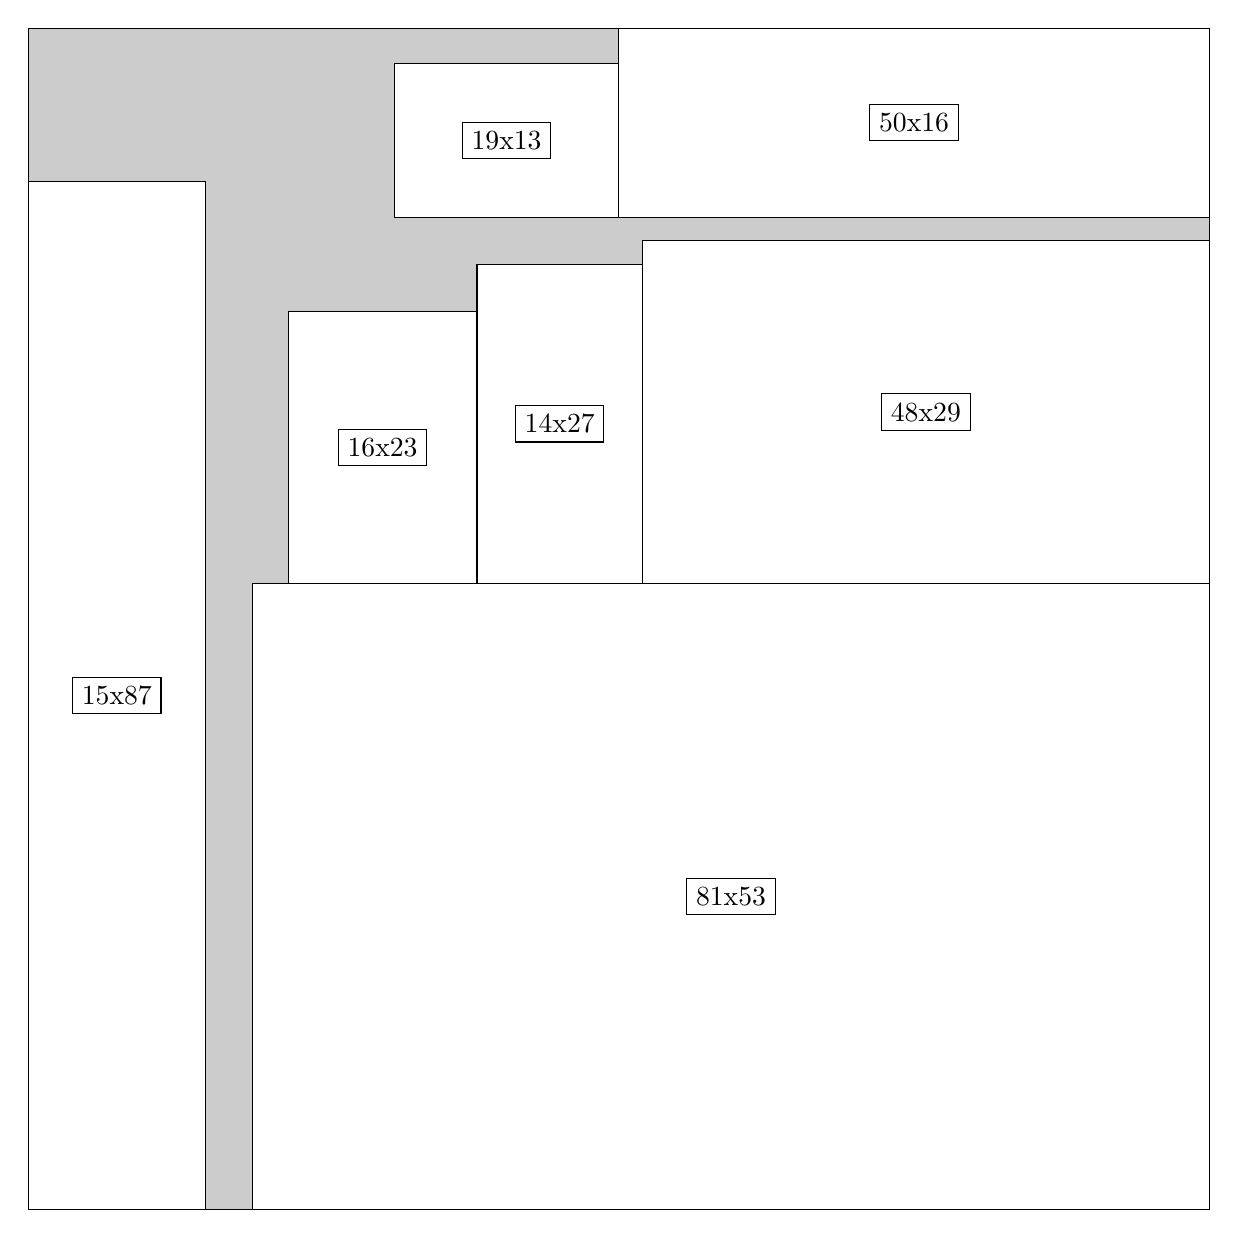
\begin{tikzpicture}[shorten >=1pt,scale=1.0,every node/.style={scale=1.0},->]
\tikzstyle{vertex}=[circle,fill=black!25,minimum size=14pt,inner sep=0pt]
\filldraw[fill=gray!40!white, draw=black] (0,0) rectangle (15.0,15.0);
\foreach \name/\x/\y/\w/\h in {81x53/2.85/0.0/12.15/7.949999999999999,48x29/7.8/7.949999999999999/7.199999999999999/4.35,14x27/5.7/7.949999999999999/2.1/4.05,16x23/3.3/7.949999999999999/2.4/3.4499999999999997,50x16/7.5/12.6/7.5/2.4,19x13/4.6499999999999995/12.6/2.85/1.95,15x87/0.0/0.0/2.25/13.049999999999999}
\filldraw[fill=white!40!white, draw=black] (\x,\y) rectangle node[draw] (\name) {\name} ++(\w,\h);
\end{tikzpicture}


w =81 , h =53 , x =19 , y =0 , v =4293
\par
w =48 , h =29 , x =52 , y =53 , v =1392
\par
w =14 , h =27 , x =38 , y =53 , v =378
\par
w =16 , h =23 , x =22 , y =53 , v =368
\par
w =50 , h =16 , x =50 , y =84 , v =800
\par
w =19 , h =13 , x =31 , y =84 , v =247
\par
w =15 , h =87 , x =0 , y =0 , v =1305
\par
\newpage


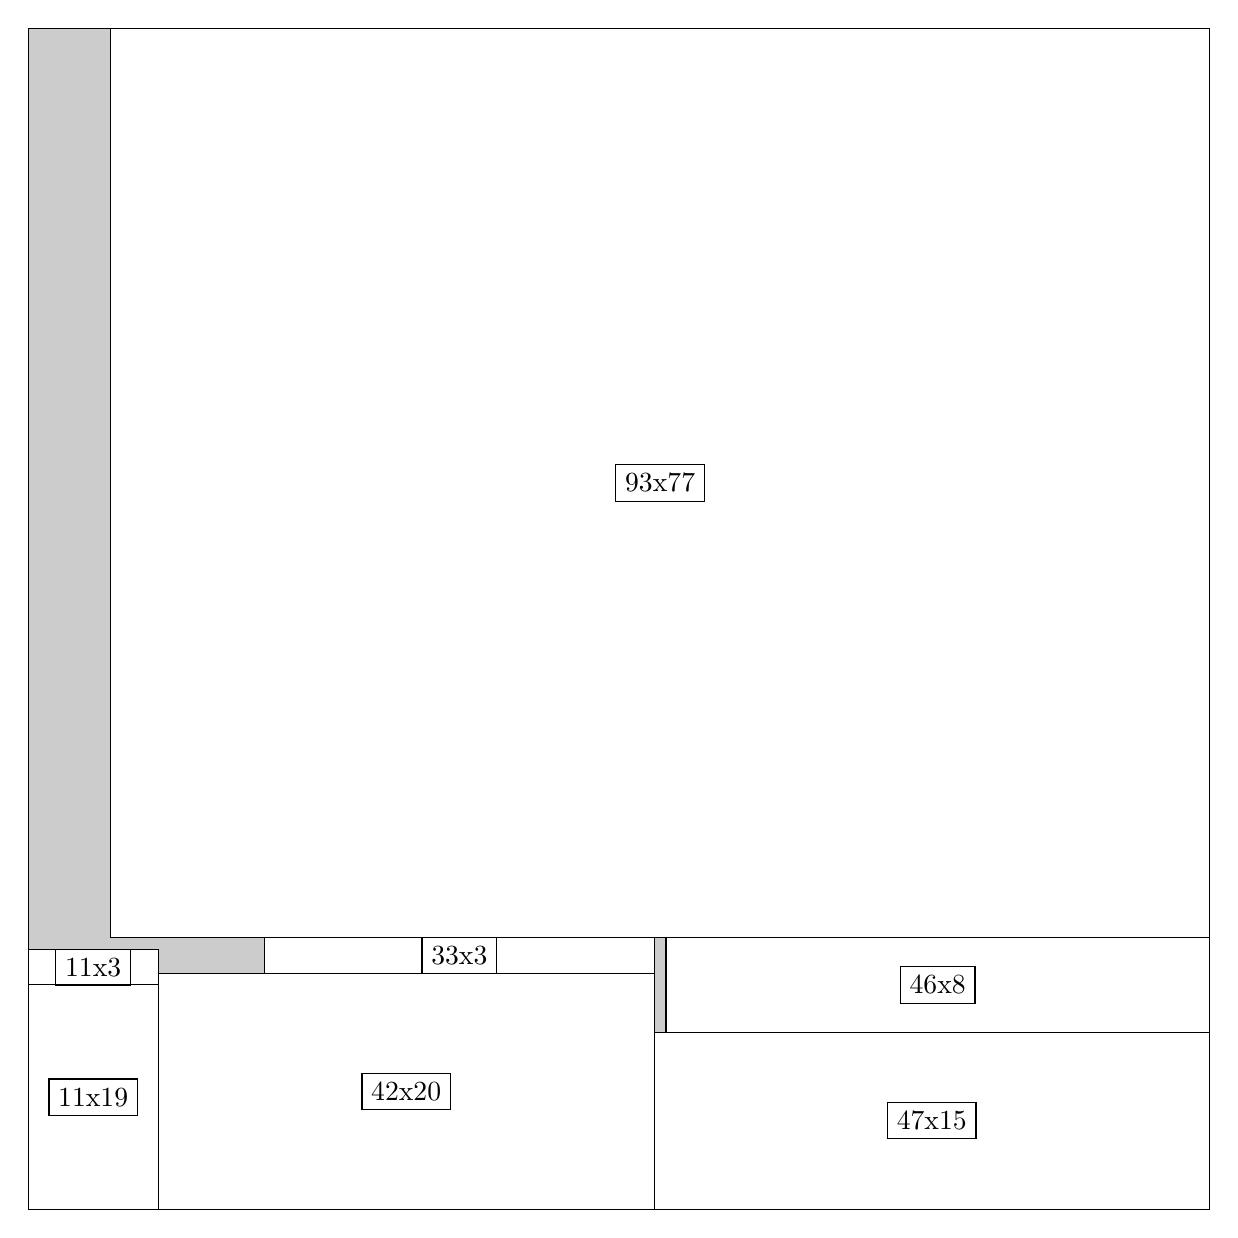
\begin{tikzpicture}[shorten >=1pt,scale=1.0,every node/.style={scale=1.0},->]
\tikzstyle{vertex}=[circle,fill=black!25,minimum size=14pt,inner sep=0pt]
\filldraw[fill=gray!40!white, draw=black] (0,0) rectangle (15.0,15.0);
\foreach \name/\x/\y/\w/\h in {47x15/7.949999999999999/0.0/7.05/2.25,46x8/8.1/2.25/6.8999999999999995/1.2,42x20/1.65/0.0/6.3/3.0,33x3/3.0/3.0/4.95/0.44999999999999996,11x19/0.0/0.0/1.65/2.85,11x3/0.0/2.85/1.65/0.44999999999999996,93x77/1.05/3.4499999999999997/13.95/11.549999999999999}
\filldraw[fill=white!40!white, draw=black] (\x,\y) rectangle node[draw] (\name) {\name} ++(\w,\h);
\end{tikzpicture}


w =47 , h =15 , x =53 , y =0 , v =705
\par
w =46 , h =8 , x =54 , y =15 , v =368
\par
w =42 , h =20 , x =11 , y =0 , v =840
\par
w =33 , h =3 , x =20 , y =20 , v =99
\par
w =11 , h =19 , x =0 , y =0 , v =209
\par
w =11 , h =3 , x =0 , y =19 , v =33
\par
w =93 , h =77 , x =7 , y =23 , v =7161
\par
\newpage


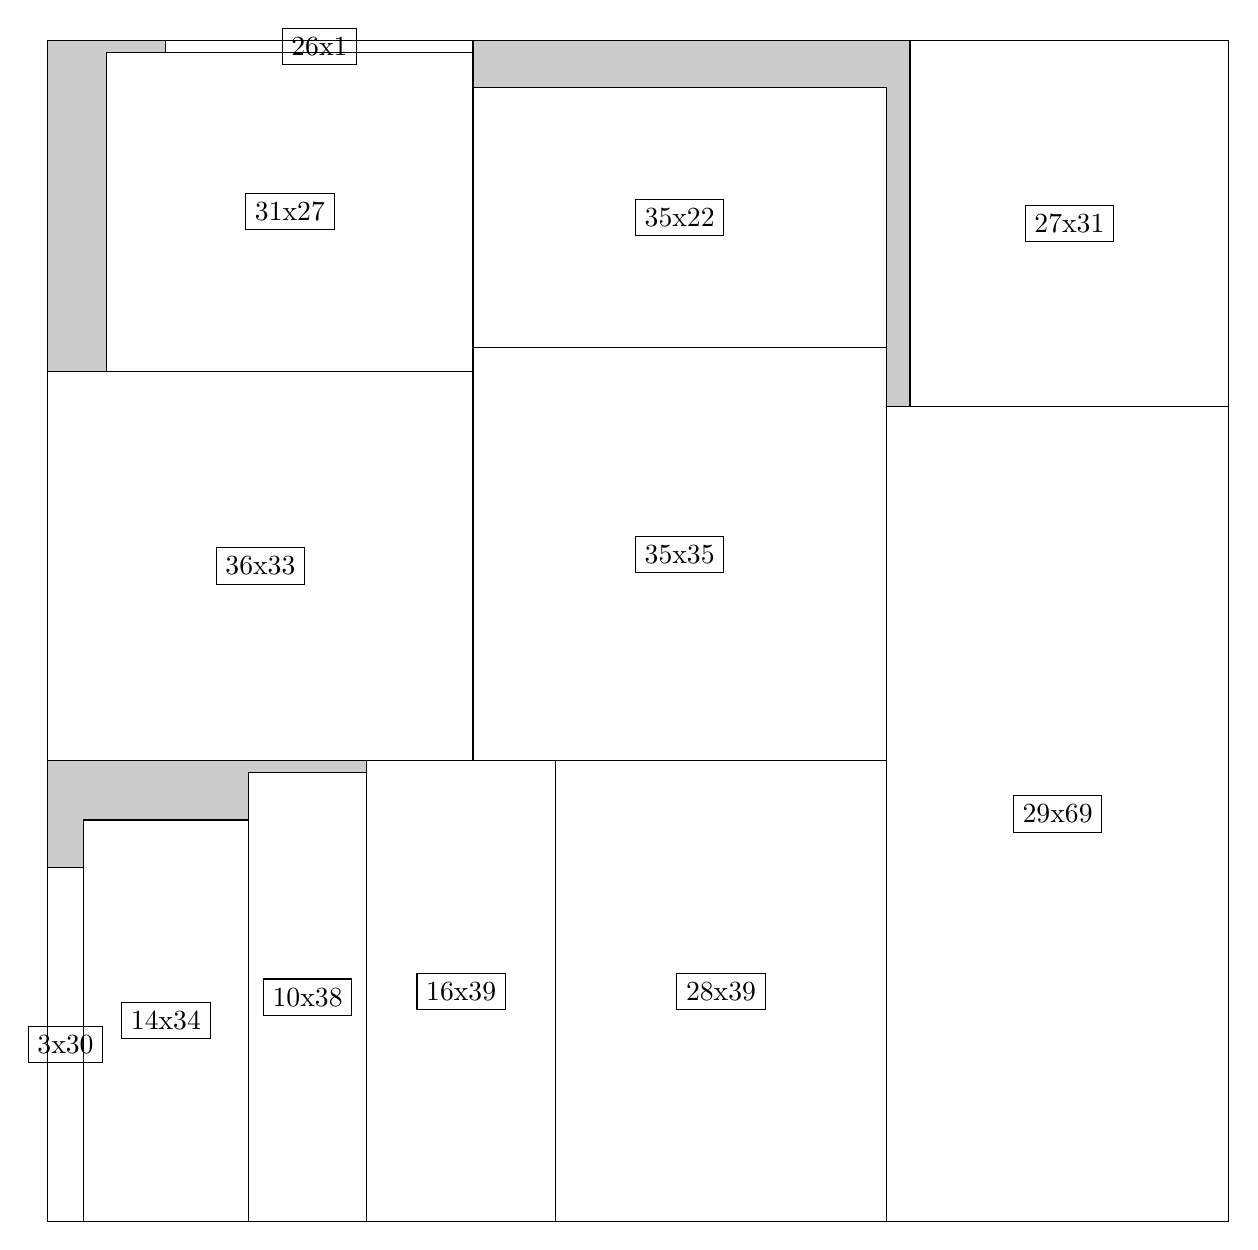
\begin{tikzpicture}[shorten >=1pt,scale=1.0,every node/.style={scale=1.0},->]
\tikzstyle{vertex}=[circle,fill=black!25,minimum size=14pt,inner sep=0pt]
\filldraw[fill=gray!40!white, draw=black] (0,0) rectangle (15.0,15.0);
\foreach \name/\x/\y/\w/\h in {29x69/10.65/0.0/4.35/10.35,27x31/10.95/10.35/4.05/4.6499999999999995,28x39/6.45/0.0/4.2/5.85,16x39/4.05/0.0/2.4/5.85,10x38/2.55/0.0/1.5/5.7,14x34/0.44999999999999996/0.0/2.1/5.1,3x30/0.0/0.0/0.44999999999999996/4.5,35x35/5.3999999999999995/5.85/5.25/5.25,35x22/5.3999999999999995/11.1/5.25/3.3,36x33/0.0/5.85/5.3999999999999995/4.95,31x27/0.75/10.799999999999999/4.6499999999999995/4.05,26x1/1.5/14.85/3.9/0.15}
\filldraw[fill=white!40!white, draw=black] (\x,\y) rectangle node[draw] (\name) {\name} ++(\w,\h);
\end{tikzpicture}


w =29 , h =69 , x =71 , y =0 , v =2001
\par
w =27 , h =31 , x =73 , y =69 , v =837
\par
w =28 , h =39 , x =43 , y =0 , v =1092
\par
w =16 , h =39 , x =27 , y =0 , v =624
\par
w =10 , h =38 , x =17 , y =0 , v =380
\par
w =14 , h =34 , x =3 , y =0 , v =476
\par
w =3 , h =30 , x =0 , y =0 , v =90
\par
w =35 , h =35 , x =36 , y =39 , v =1225
\par
w =35 , h =22 , x =36 , y =74 , v =770
\par
w =36 , h =33 , x =0 , y =39 , v =1188
\par
w =31 , h =27 , x =5 , y =72 , v =837
\par
w =26 , h =1 , x =10 , y =99 , v =26
\par
\newpage


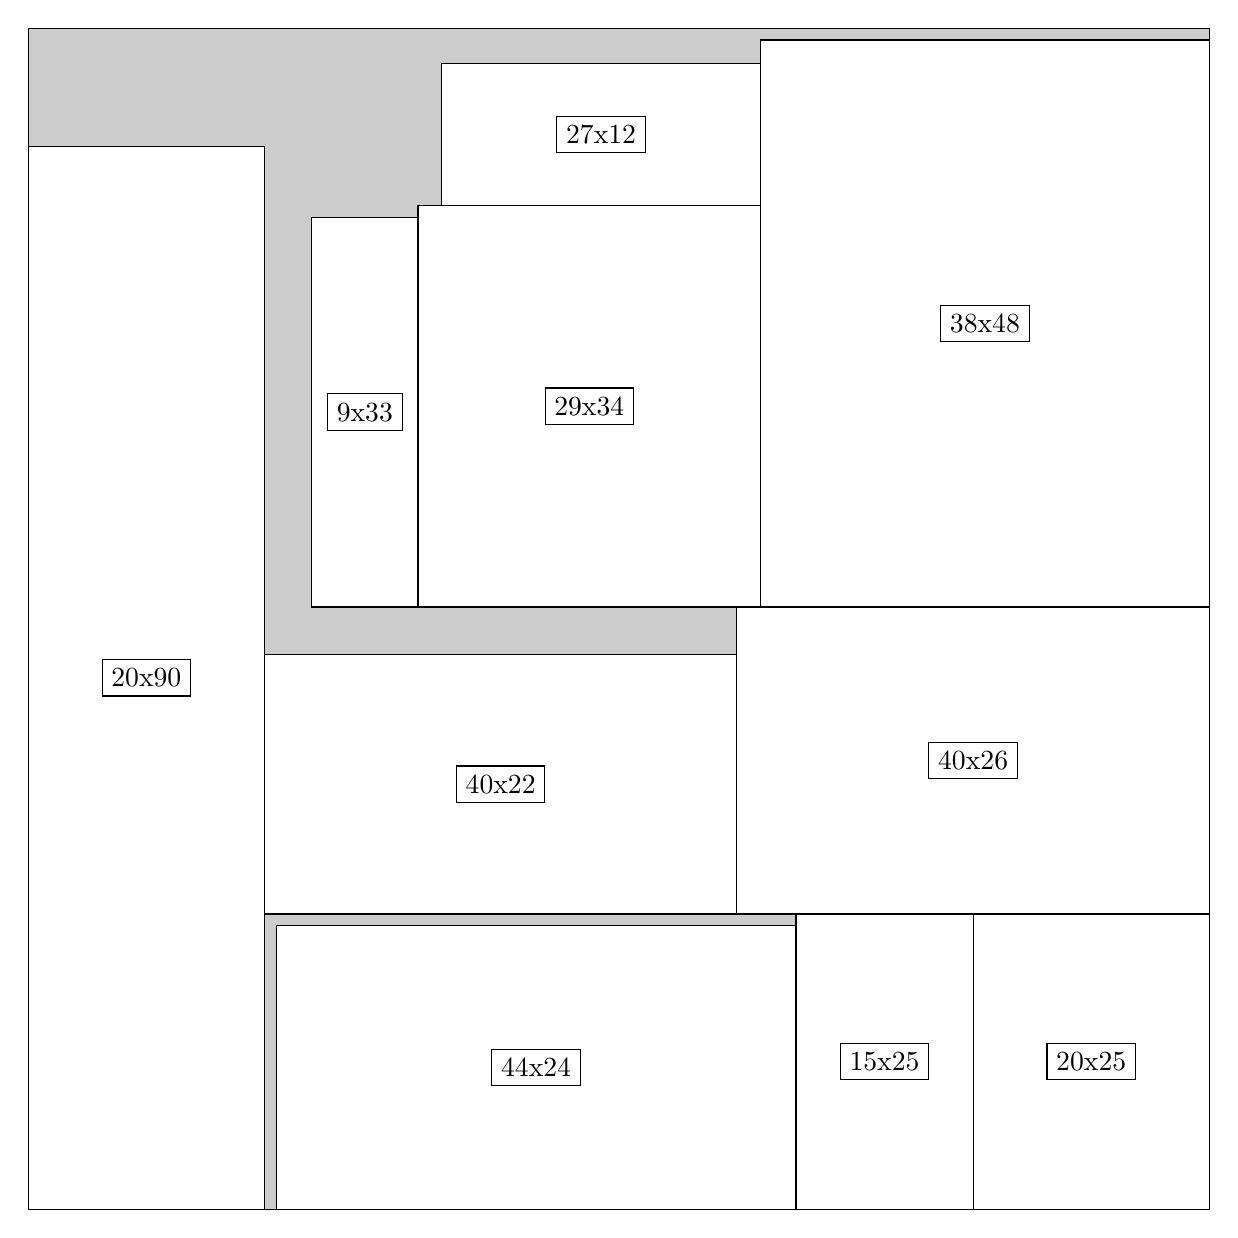
\begin{tikzpicture}[shorten >=1pt,scale=1.0,every node/.style={scale=1.0},->]
\tikzstyle{vertex}=[circle,fill=black!25,minimum size=14pt,inner sep=0pt]
\filldraw[fill=gray!40!white, draw=black] (0,0) rectangle (15.0,15.0);
\foreach \name/\x/\y/\w/\h in {20x25/12.0/0.0/3.0/3.75,15x25/9.75/0.0/2.25/3.75,44x24/3.15/0.0/6.6/3.5999999999999996,40x26/9.0/3.75/6.0/3.9,40x22/3.0/3.75/6.0/3.3,38x48/9.299999999999999/7.6499999999999995/5.7/7.199999999999999,29x34/4.95/7.6499999999999995/4.35/5.1,27x12/5.25/12.75/4.05/1.7999999999999998,9x33/3.5999999999999996/7.6499999999999995/1.3499999999999999/4.95,20x90/0.0/0.0/3.0/13.5}
\filldraw[fill=white!40!white, draw=black] (\x,\y) rectangle node[draw] (\name) {\name} ++(\w,\h);
\end{tikzpicture}


w =20 , h =25 , x =80 , y =0 , v =500
\par
w =15 , h =25 , x =65 , y =0 , v =375
\par
w =44 , h =24 , x =21 , y =0 , v =1056
\par
w =40 , h =26 , x =60 , y =25 , v =1040
\par
w =40 , h =22 , x =20 , y =25 , v =880
\par
w =38 , h =48 , x =62 , y =51 , v =1824
\par
w =29 , h =34 , x =33 , y =51 , v =986
\par
w =27 , h =12 , x =35 , y =85 , v =324
\par
w =9 , h =33 , x =24 , y =51 , v =297
\par
w =20 , h =90 , x =0 , y =0 , v =1800
\par
\newpage


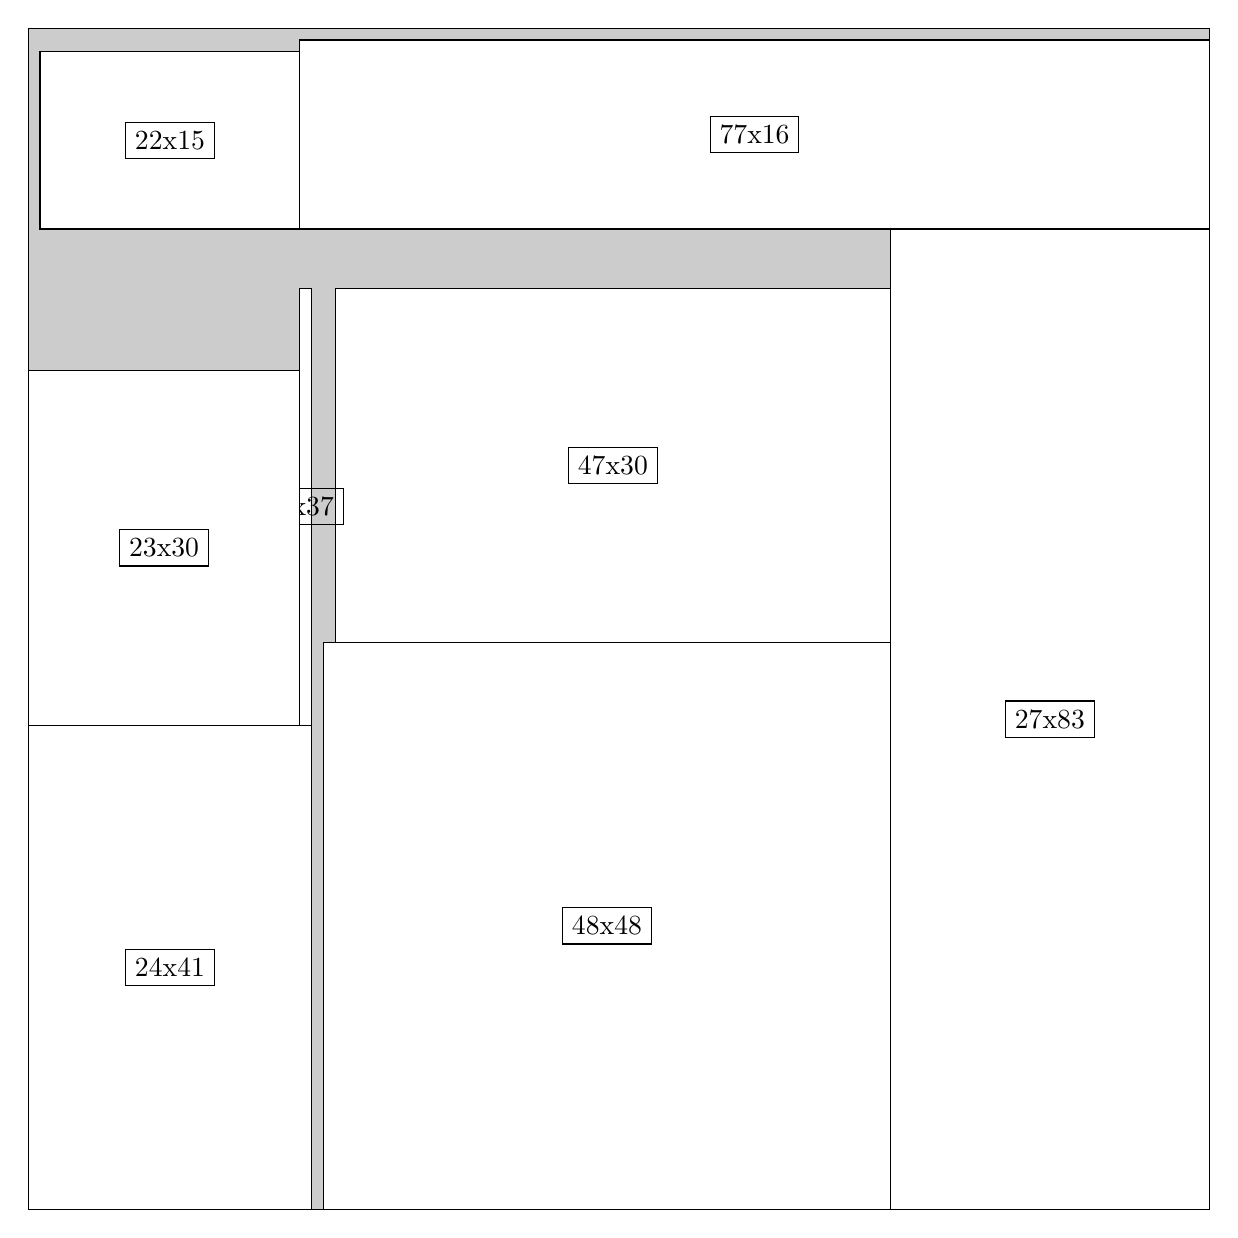
\begin{tikzpicture}[shorten >=1pt,scale=1.0,every node/.style={scale=1.0},->]
\tikzstyle{vertex}=[circle,fill=black!25,minimum size=14pt,inner sep=0pt]
\filldraw[fill=gray!40!white, draw=black] (0,0) rectangle (15.0,15.0);
\foreach \name/\x/\y/\w/\h in {27x83/10.95/0.0/4.05/12.45,48x48/3.75/0.0/7.199999999999999/7.199999999999999,47x30/3.9/7.199999999999999/7.05/4.5,24x41/0.0/0.0/3.5999999999999996/6.1499999999999995,1x37/3.4499999999999997/6.1499999999999995/0.15/5.55,23x30/0.0/6.1499999999999995/3.4499999999999997/4.5,77x16/3.4499999999999997/12.45/11.549999999999999/2.4,22x15/0.15/12.45/3.3/2.25}
\filldraw[fill=white!40!white, draw=black] (\x,\y) rectangle node[draw] (\name) {\name} ++(\w,\h);
\end{tikzpicture}


w =27 , h =83 , x =73 , y =0 , v =2241
\par
w =48 , h =48 , x =25 , y =0 , v =2304
\par
w =47 , h =30 , x =26 , y =48 , v =1410
\par
w =24 , h =41 , x =0 , y =0 , v =984
\par
w =1 , h =37 , x =23 , y =41 , v =37
\par
w =23 , h =30 , x =0 , y =41 , v =690
\par
w =77 , h =16 , x =23 , y =83 , v =1232
\par
w =22 , h =15 , x =1 , y =83 , v =330
\par
\newpage


\end{document}